\documentclass[a4paper, 12pt]{report}

\usepackage[utf8]{inputenc}
\usepackage{amssymb}           % dodatni simboli
\usepackage[slovene,english]{babel}    % naloži, med drugim, slovenske delilne vzorce
\usepackage[pdftex]{graphicx}  % omogoča vlaganje slik različnih formatov
\usepackage[round]{natbib}
\usepackage{fancyhdr}          % poskrbi, na primer, za glave strani
% robovi: nastavljeno je na top=35mm bottom=30mm left,right=25mm
\usepackage[a4paper, top=30mm, bottom=35mm,left=25mm,right=25mm]{geometry} 
\usepackage[nottoc,numbib]{tocbibind} % za stevilko poglavja "viri"

\usepackage{mathptmx}       % font: Times New Roman
\linespread{1.15}           % razmak med vrsticami
\setlength{\parskip}{1em}   % razmak med odstavki (popravljeno v kazalu)
\setlength{\parindent}{0pt} % brez indentacije

\usepackage{hyperref}       % povezave v kazalu
\hypersetup{
    colorlinks,
    citecolor=black,
    filecolor=black,
    linkcolor=black,
    urlcolor=black
}

%% POGLAVJA
\setcounter{secnumdepth}{3} % 4 stopnje poglavij
\usepackage{titlesec} % popravki naslovov poglavij
% nastavitve za chapter
\titleformat{\chapter}[hang]{\bfseries\MakeUppercase}{\thechapter}{30pt}{} 
\titlespacing{\chapter}{0pt}{-2.5em}{0em}
\assignpagestyle{\chapter}{fancy}

% nastavitve za section
\titleformat{\section}[hang]{\MakeUppercase}{\thesection}{21pt}{} 
\titlespacing{\section}{0pt}{1em}{0em}

% nastavitve za subsection
\titleformat{\subsection}[hang]{\bfseries}{\thesubsection}{12pt}{} 
\titlespacing{\subsection}{0pt}{0pt}{0pt}

% nastavitve za subsubsection
\titleformat{\subsubsection}{\normalfont\normalsize}{\thesubsubsection}{3pt}{}

%% HEADER, FOOTER
\pagestyle{fancy}
\fancyhf{}
\lhead{\small Novak, Janez. Vzorec zaključnega dela na biotehniški fakulteteti\\
Univerza v Ljubljani, Biotehniška fakulteta, 2020}
\rhead{\thepage}

% KAZALO

\setcounter{tocdepth}{3} % v kazalu pokazi 4 stopnji
\addto\captionsslovene{
  \renewcommand{\contentsname}{\vskip 2em \hfill Kazalo vsebine\hfill}
}

% LITERATURA IN VIRI

\addto\captionsslovene{
  \renewcommand{\bibname}{Viri}
}

%% METADATA

\author{Janez Novak}
\date{oktober 2020}

% ZACETEK DOKUMENTA

\begin{document}

\selectlanguage{slovene}
\newcommand{\sn}[1]{"`#1"'}     % slovenski narekovaji

\pagenumbering{Roman}

%%%%%%%%%%%%%%%%%%%%%%%%%%%%%%%%%%%%%%%%
% NASLOVNICA
\thispagestyle{empty}%
\begin{titlepage}
\makeatletter

\begin{center}
{\Large\sc UNIVERZA V LJUBLJANI\\%
BIOTEHNIŠKA FAKULTETA\\%
}

\vskip 10em%

{\ \LARGE \\
    VZOREC ZAKLJUČNEGA DELA NA \\
    BIOTEHNIŠKI FAKULTETETI
\par}%
{\ \Large Seminarska naloga z uporabo \LaTeX a \\
\par}%
\end{center}

\vskip 15em%

\noindent\textbf{Ime in priimek:} \@author \\
\noindent\textbf{Študijski program:} Ekologija in biodiverziteta\\
\noindent\textbf{Mentor:} Dr. Alenka Hrastnik\\

\vskip 5em%

\begin{center}
Ljubljana, \@date
\end{center}
\end{titlepage}

\setcounter{page}{2}

%% Kazalo

\setlength{\parskip}{0em}
\tableofcontents
\setlength{\parskip}{1em}

%% Zacetek vsebine

\clearpage\pagenumbering{arabic}

\chapter{Uvod}

Prvi koristen nasvet v zvezi uporabo \LaTeX{a} je, da v celoti preberete ta dokument!

Datoteka {\tt vzorec.tex} na kratko opisuje, kako se pisanja diplomskega dela lotimo z uporabo programskega okolja \LaTeX.
V tem dokumentu bomo predstavili nekaj njegovih prednosti in hib. 
Kar se slednjih tiče, nam pride na misel ena sama. 
Ko se srečamo z njim prvič, nam izgleda morda kot kislo jabolko, nismo prepričani, ali bi želeli vanj ugrizniti. 
Toda prav iz kislih jabolk lahko pripravimo odličen jabolčni zavitek in s praktičnim preizkusom \LaTeX a najlažje pridemo na njegov pravi okus.


\LaTeX\ loči vsebino dokumneta od njegovega formata, kar ima v primerjavi z vizualnim urejanjem številne prednost.
Omogoča večjo konsistentnost, uniformnost in prenosljivost besedil. 

Ta vzorec definira format, ki ga opisujejo Navodila za pripravo zaključnih pisnih izdelkov na Biotehniški fakulteti (\url{http://www.bf.uni-lj.si/fileadmin/users/1/knjiznice/Navodila_za_pripravo_zakljucnih_pisnih_izdelkov_na_BF.pdf}). Format (še) ni popolnoma pravilen, bi pa moral zadostovati seminarskim nalogam.

\chapter{Kako začeti}

\section{Overleaf}

Najbolj enostaven način, kako se lotimo učenja \LaTeX a, je spletna aplikacija Overleaf (\url{http://overleaf.com}). Če so Google Docs online verzija Microsoft Word-a, je Overleaf online verzija \LaTeX-a.

\begin{enumerate}
  \item Ustvari Overleaf račun.
  \item Ustvari nov prazen projekt.
  \item Vanj prenesi datoteke: \texttt{vzorec.tex}, \texttt{viri.bib} in \texttt{bib-style.bst}.
\end{enumerate}

\begin{figure}[h]
\begin{center}
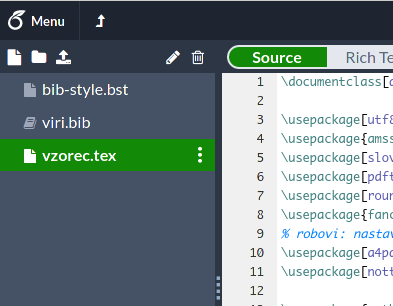
\includegraphics[width=0.6\textwidth]{images/overleaf-sidebar.png}
\end{center}
\caption{Tako bi morale izgledati datoteke v novem Overleaf projektu.}
\label{pic1}
\end{figure}

\section{Pisanje vsebine}

Če odpremo datoteko \texttt{vzorec.tex} lahko vidimo, da vsebuje:

\begin{itemize}
  \item veliko neke "kode" na začetku in
  \item besedilo tega dokumenta na koncu.
\end{itemize}

Če v drugi del datoteke začnemo pisati svojo vsebino in pritisnemo gumb "Recompile", bi se moral ta dokument na desni posodobiti.

\chapter{Kako naredim \_?}

\section{Naslov}

\LaTeX ima na voljo 4 stopenj naslovov:

\begin{enumerate}
  \item \texttt{\textbackslash chapter\{Moj naslov 1. stopnje\} }
  \item \texttt{\textbackslash section\{Moj naslov 2. stopnje\} }
  \item \texttt{\textbackslash subsection\{Moj naslov 3. stopnje\} }
  \item \texttt{\textbackslash subsubsection\{Moj naslov 4. stopnje\} }
\end{enumerate}

Obstajajo tudi naslovi odstavkov: \texttt{\textbackslash paragraph\{Moj odstavek\} }

\section{Seznam}

\begin{verbatim}
\begin{itemize}
  \item Prva neostevicena alineja
  \item Druga neostevicena alineja
\end{itemize}
\end{verbatim}

\begin{verbatim}
\begin{enumarate}
  \item Prva ostevicena alineja
  \item Druga ostevicena alineja
\end{enumarate}
\end{verbatim}

\section{Različne pisave}
 
\begin{verbatim}
Text, ki ga označim \textbf{takole}, je odebeljen, 
\textit{takole} pa je postrani.
\end{verbatim}

\newpage

\section{Citat}

Če želim citirati, moram v datoteko \texttt{viri.bib} dodati vnos oblike:

\begin{verbatim}
@article{Dolinar2019,
  author = {Dolinar, Katja and Krajnik, Matej},
  year = {2019},
  title = {{Priročnik za terensko delo na Krasu}},
  journal = {Ljubljana, Gozdarski inštitut Slovenije},
  volume = {Silva Slovenica},
  pages = {106--107},
}  
\end{verbatim}

V besedilu uporabim \texttt{\textbackslash citep\{Dolinar2019\} } in citat bo izgledal takole: \citep{Dolinar2019}

Če je vnos v \texttt{viri.bib} pravilne oblike, bi se moral na koncu dokumenta pojaviti v poglavju "Viri".

\bibliographystyle{bib-style}
\bibliography{viri}

\end{document}
